\documentclass[12pt]{article}
\usepackage[left=2cm, right=2cm, top=2cm]{geometry}
\usepackage[utf8]{inputenc} 
\usepackage{mdframed} %For framing the title
\usepackage{graphicx} % to include images
\usepackage{amsmath} % For math mode
\usepackage{mathtools} %for bmatrix*
\usepackage{caption} % For captions
\usepackage{subcaption} % To use caption while using mini page
\usepackage{amssymb} % To use math symbols
\usepackage{multirow} %To combine multiple rows in a table
\usepackage[table]{xcolor} %To color rows / columns in table
\usepackage{titling} %To vertically center the title page
\usepackage{hyperref} %for URL
\usepackage{float} %For [H] in includegraphics
\usepackage[section]{placeins} %PRevents floats before a section
\usepackage{textcomp} %For degree symbol
\usepackage[none]{hyphenat} %To prevent hyphens



%----------------------------MATLAB TEMPLATE -------------------------------------
\usepackage{listings}
\usepackage{color} %red, green, blue, yellow, cyan, magenta, black, white
\definecolor{mygreen}{RGB}{28,172,0} % color values Red, Green, Blue
\definecolor{mylilas}{RGB}{170,55,241}
%-----------------------------------------------------------------------------------------

\title{ECE 8540 \\ Analysis of Tracking Systems \\ \quad \\
	Assignment 7 \\ Particle Filter}
\author{Vivek Koodli Udupa \\ C12768888}
\date{November 29, 2018 }

%%To make the title page center vertically centered
%\renewcommand\maketitlehooka{\null\mbox{}\vfill}
%\renewcommand\maketitlehookd{\vfill\null}

\begin{document}
\begin{mdframed}
%Displaying Title
%\begin{titlepage}
\maketitle
%\pagenumbering{gobble}% Remove page numbers (and reset to 1)
%\end{titlepage}
\end{mdframed}
\pagenumbering{arabic}% Arabic page numbers (and reset to 1)


%Begin of Report
\section{Introduction}
This report considers the problem of modeling a system described by Hidden Markov Model(HMM). A Markov model is a stochastic model used to model randomly changing systems. A Markov process is a random process where the future state is independent of the past states given the present state. A Hidden Markov Model is a statistical Markov model in which the system being modeled is assumed to be a Markov process with unobserved (i.e. hidden) states. The aim is to discover the hidden state
sequence that most likely describes a given observation sequence. \\

One solution to this problem is to use the Viterbi algorithm, which finds the single best state sequence for an observation sequence. For example, in speech-to-text (speech recognition), the acoustic signal is treated as the observed sequence of events, and a string of text is considered to be the \lq\lq{hidden cause}\rq\rq{} of the acoustic signal. The Viterbi algorithm finds the most likely string of text given the acoustic signal.  \\

The problem considered for this report is a simple HMM which comprises of two states, H(High GC content) and L(Low GC content). State H characterizes coding DNA while state L characterizes non-coding DNA. The model is used to predict the region of coding DNA from a given sequence. 

\section{Methods}
This section describes the implementation of the Viterbi algorithm to find the hidden state probabilities for the given problem. \\

The HMM in consideration is shown in Figure \ref{fig:HMM}. The model consists of two states, labeled H and L in the example, which can be given numerical values of 0 and 1. The prior probabilities are {0.5, 0.5}. The state transition
probabilities are {0.5, 0.5} for state 0 and {0.4, 0.6} for state 1. Each state observes a discrete value that takes on one of four values {A, C, G, T } that can be given numerical values {0, 1, 2, 3}. The emission probabilities of these values are {0.2, 0.3, 0.3, 0.2} for state 0 and {0.3, 0.2, 0.2, 0.3} for state 1.
 
 \begin{figure}[H]
	\centering
	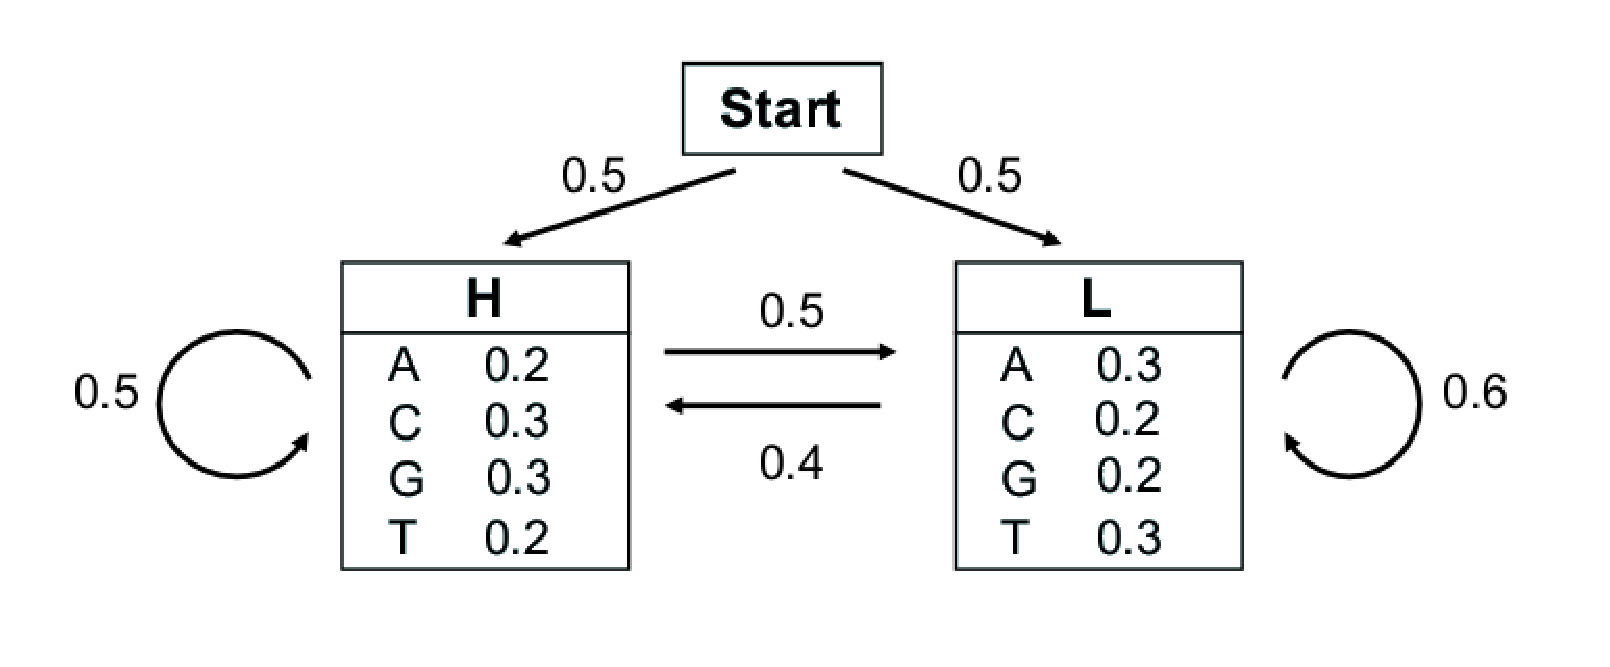
\includegraphics[scale=0.5]{HMM.eps}
	\caption{The Hidden Markov Model with H and T States}
	\label{fig:HMM}
\end{figure}

The Viterbi calculations are done using sums of $log_2$ probabilities. \\

There are several paths that lead to the desired sequence of states, but not all of them have the same probabilities. The Viterbi algorithm is a dynamical programming algorithm that computes the most probable path. \\

The probability of the most probable path ending in state k with observation \lq\lq{ i }\rq\rq{} is: 
\begin{equation}
	p_l(i,x) = e_l(i) \cdot \displaystyle\max_k(p_k(j,x-1) \cdot p_{kl})
\end{equation}





\section{Results}

\section{Conclusion}

\section*{References}

\section*{Appendix}

\subsection*{MATLAB Code}
%\lstinputlisting{../asg6.m}
%--------------------------------------------------------------------------------------------------------

\end{document}